\section{Numerical experiments}\label{sec:numerics}

In this section we verify numerically that the order of the constructed Runge-Kutta scheme $TM^{n}R$\yianniscomment{IOn section 5 }, for which the main method $M$ is an SSPRK($s$,$q$,$p$) method, is the effective order $q$ of method $M$. This is done by performing a convergence study on a smooth nonlinear problem. Also we show that the $TM^{n}R$ scheme inherits the properties of the SSPRK($s$,$q$,$p$) method. In particular, the time-step restriction of the Runge-Kutta scheme $TM^{n}R$ is the same with that of the main method $M$. This is demonstrated by showing the effect of SSP coefficient on the nonlinear Burger's equation.

\subsection{Convergence study}\label{subsec:convergence}

We consider the nonlinear equation
\begin{equation}\label{eq5.3}
    u'(t) = -\frac{3}{2}u^{2}(t), \quad t \in [0,1], \quad \text{with } u(0) = 10,
\end{equation}
and exact solution
\begin{equation}\label{eq5.4}
    u(t) = 10/(15t + 1).
\end{equation}
We solve the initial value problem \eqref{eq5.3} and \eqref{eq5.4} using an $TM^{n}R$ Runge-Kutta scheme, where $M$ is a $q$-effective order SSPRK method for $q = 3, 4$. 
Method $M$ was found by solving the optimisation problem \eqref{eq5.2} and the starting and finishing methods were found by solving the problem \eqref{eq5.3}. 
The stages of the permutation methods were kept as low as possible, thus we use two stages for a 3-effective order method $M$ and four stages for a 4-effective order method. 
The solution is computed for $N = 50.2^{k}$ for $k = 0, 1, 2, \dots, 6$ and hence the time-step used is $\Dt = \frac{1}{N} = \frac{2^{1-N}}{100}$ for each computation. 
The error between the exact solution and the approximation with respect to time-step is shown in Figures \ref{fig5.1} and \ref{fig5.2} on a logarithmic scale. \yiannistodo{Update pictures, correct legends, axis, etc.}
The convergence study was performed for various stages and the results show that the Runge-Kutta scheme $TM^{n}R $ attends order equal to the effective order of method $M$. 
We note it is important to measure the error after applying the finishing method $R$, otherwise we observe the
classical order $p$ of method $M$ instead of the higher effective order $q$. 
Finally, we note that for a fixed time-step, increasing the number of stages the decreases the error.

\begin{figure}[t!]
    \centering
    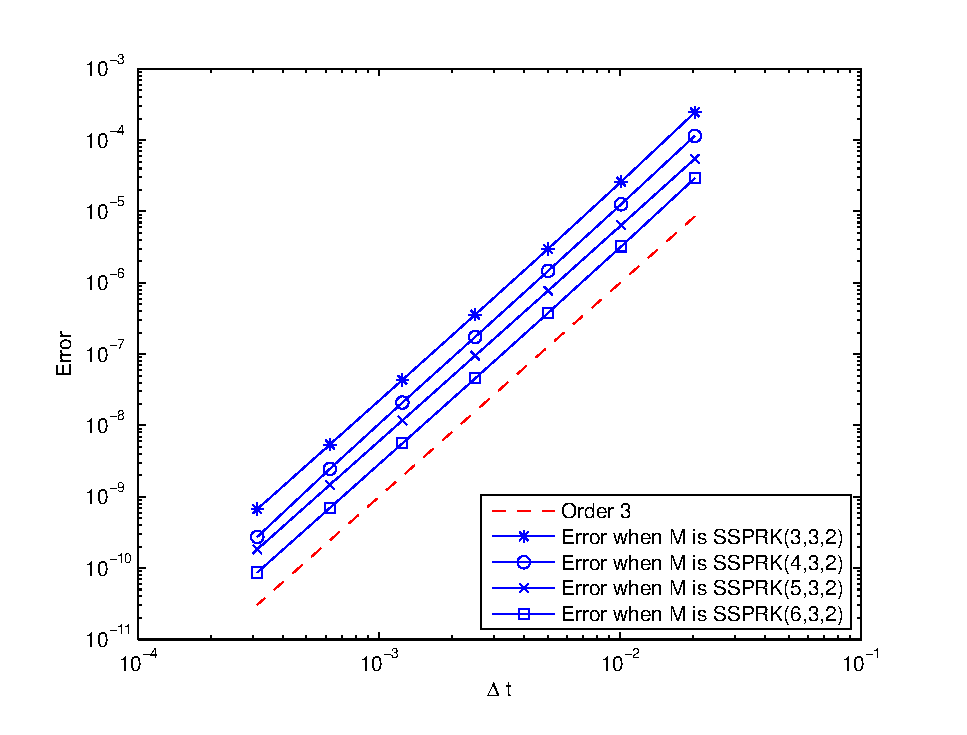
\includegraphics[scale=0.6]{Pictures/convergence_3rd_ord.eps}
    \caption{Convergence of $ SM^{n}S^{-1} $ Runge-Kutta scheme, when $ M $ is SSPRK($ s $,$ 3 $,$ 2 $) method.}
    \label{fig5.1}
\end{figure}

\begin{figure}[t!]
    \centering
    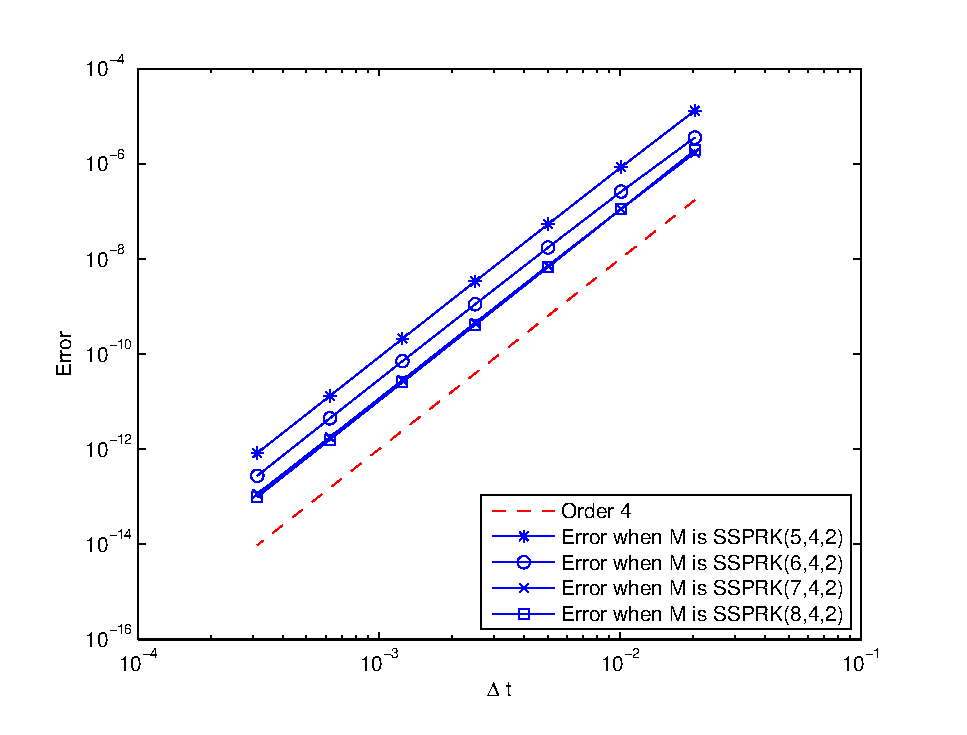
\includegraphics[scale=0.6]{Pictures/convergence_4th_ord_(1).eps}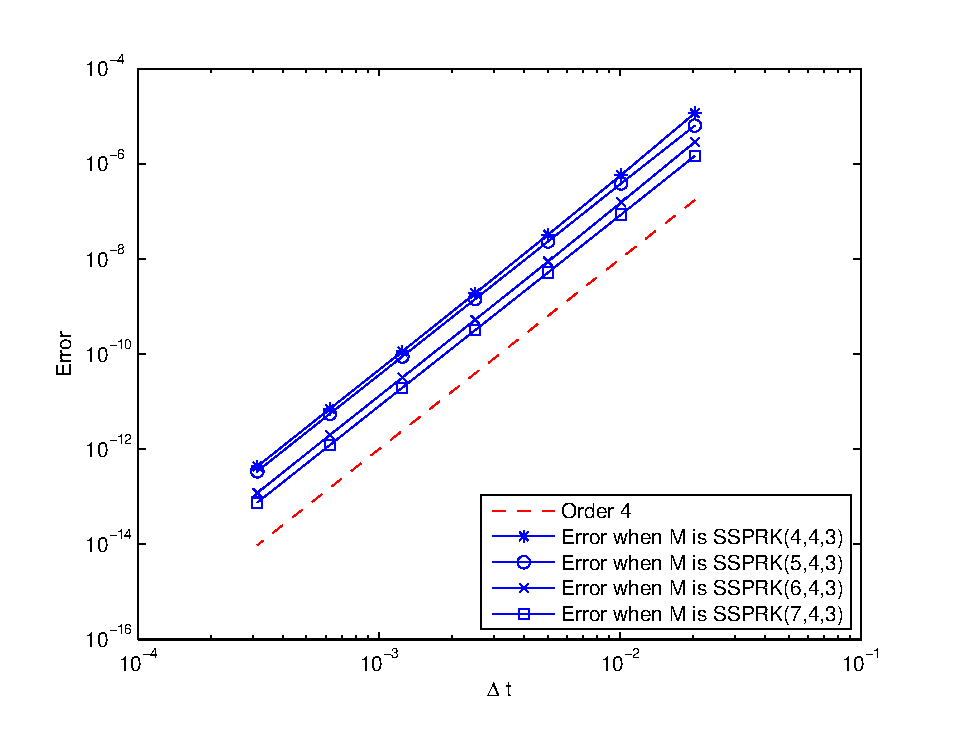
\includegraphics[scale=0.6]{Pictures/convergence_4th_ord_(2).eps}
    \caption{Convergence of $TM^{n}R$ Runge-Kutta scheme when (a) $M$ is SSPRK($s $,$ 4 $,$ 2 $) method and (b) $ M $ is SSPRK($ s $,$ 4 $,$ 3 $) method.}
    \label{fig5.2}
\end{figure}

\subsection{Application to nonlinear problems}\label{subsec:nonlinear_problems}

\subsubsection{Burger's equation}\label{subsubsec:burgers}

The inviscid Burger's equation consists of the hyperbolic conservation law
\begin{equation}\label{eq5.5}
    U_{t} + f(U)_{x} = 0,
\end{equation}
when the flux function $f(U) = \frac{1}{2}U^{2}$. We consider initial data
\begin{equation}\label{eq5.6}
    u(0,x)  = \frac{1}{2} - \frac{1}{4}sin{\pi x},
\end{equation}
on a periodic domain $x \in [0,2)$. The solution advances to the right where it eventually exhibits a shock. We perform a semi-discetisation of $f(U)_{x}$ using an upwind approximation \cite{Ketcheson2009} that gives
\begin{equation}\label{eq5.7}
    f(U)_{x} \approx \frac{1}{\Dt}\bigl(f(u_{i}) - f(u_{i-1})\bigr).
\end{equation}

The above time discretisation is SSP when coupled with Forward Euler method under time restriction $\Dt \leq {\Dt}_{FE} = \frac{\Delta x}{\|u(0,x)\|_{\infty}}$. We integrate to time $t_{f} = 2.3$ with $m = 256$ points in space.
\newline

\begin{figure}[t!]
    \centering
    \subfloat[$\sigma = 6.0$]{\label{fig5.3a}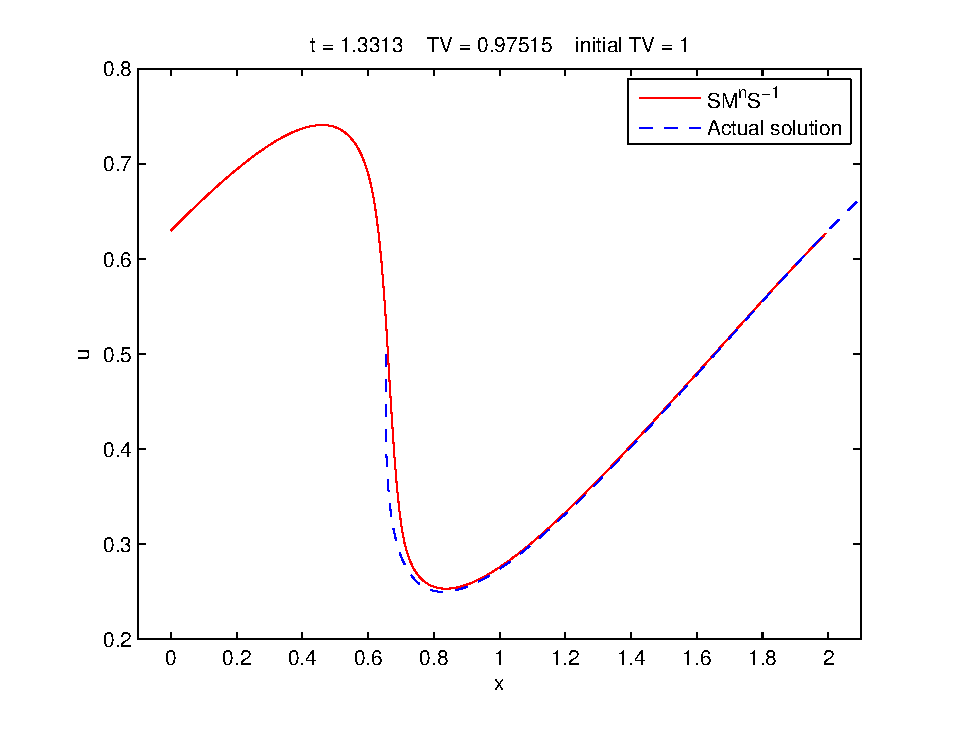
\includegraphics[scale=0.7]{Pictures/burgers_cont_tvd.eps}} \\
    \subfloat[$\sigma = 7.1$]{\label{fig5.3b}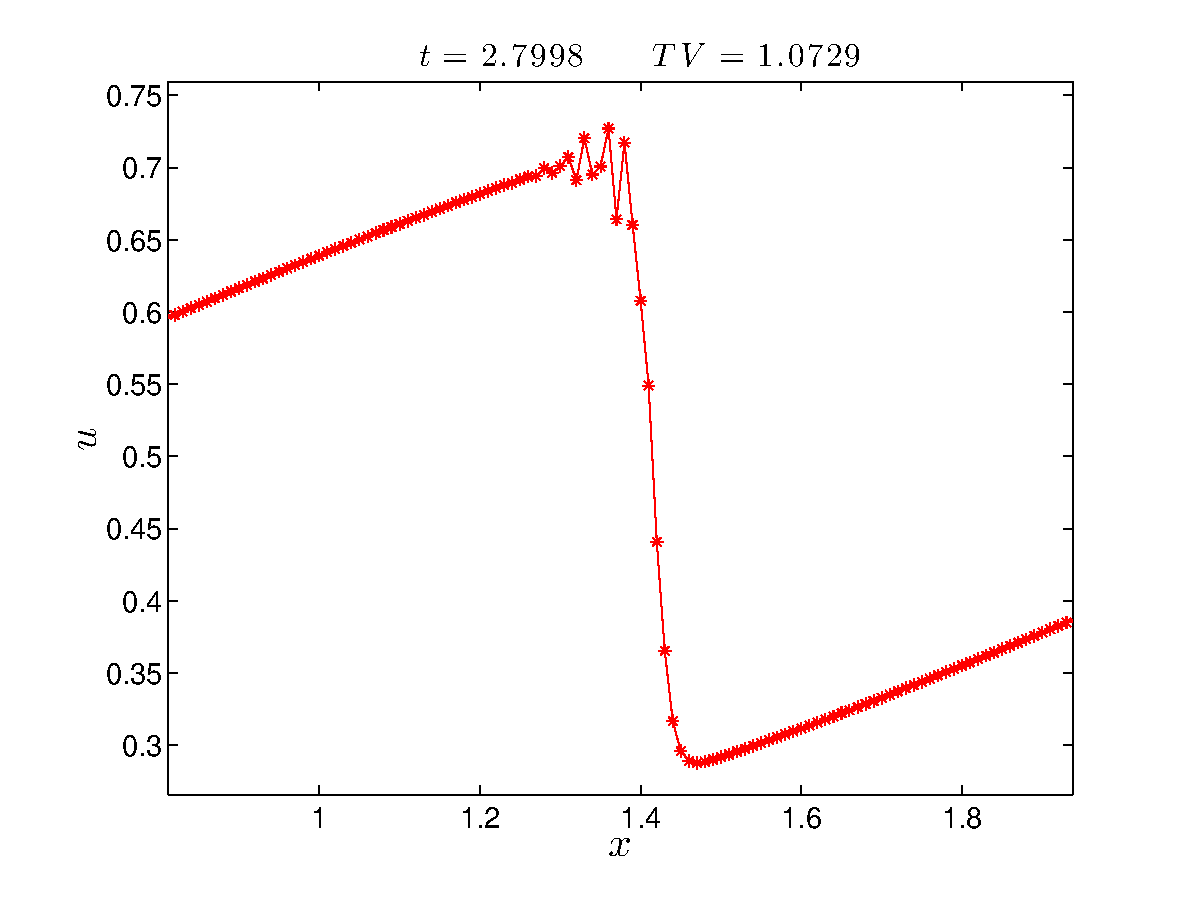
\includegraphics[scale=0.7]{Pictures/burgers_cont_no_tvd.eps}}
    \caption{Solution of Burger's equation with continuous initial data, using a $ SM^{n}S^{-1} $ scheme, where $ M $ is SSPRK($ 10 $,$ 4 $,$ 3 $). The SSP coefficient is $ c = 6.0 $.}
    \label{fig5.3}
\end{figure}

Burger's equation was solved using a $TM^{n}R$ Runge-Kutta scheme with time-step restriction $\Dt \leq \sigma{\Dt}_{FE}$, where $\sigma$ indicates the size of the time step. Figure \ref{fig5.3} shows that if $\sigma$ stays below the SSP coefficient of the method $M$, then no oscillations are observed. If this stability limit is violated, then oscillations appear. \yianniscomment{Elaborate more: Sharpness of SSP coefficient} We were able to determine when exactly the nonlinear stability is not satisfied by computing the the total-variation (TV) norm at each step of the computation process. This indicates that the $TM^{n}R$ scheme inherits the time-step restriction from the SSP coefficient of the main method $M$.
\newline

We also consider Burger's equation with discontinuous data
\begin{equation}\label{eq5.8}
    u(0,x)  = \left\{
                \begin{array}{ll}
                  1, & \hbox{$0.5 \leq x \leq 1.5$} \\
                  0, & \hbox{otherwise.}
                \end{array}
              \right.
\end{equation}

Figure \ref{fig5.4} shows the result of solving the discontinuous problem using a $TM^{n}R$ Runge-Kutta scheme, with $M$ an SSPRK($4$,$4$,$3$). Clearly, the monotonicity in the TV-norm is violated at $t = 0$ because the method $S$ is not an SSP method. However, this does not propagate in time if the time-step size $\sigma$ is kept below the SSP coefficient of method $M$. Otherwise, oscillations continue to appear for $t > 0$. The actual solution was plotted using the method of the characteristics and is given by

\begin{equation}\label{eq5.9}
    u(t,x)  = \left\{
                \begin{array}{ll}
                  0, & \hbox{$0 \leq x \leq 0.5$} \\
                  \frac{x-0.5}{t}, & \hbox{$0.5 < x \leq 0.5 + t$} \\
                  1, & \hbox{$0.5 + t < x \leq 1.5  + \frac{t}{2}$} \\
                  0, & \hbox{$1.5  + \frac{t}{2} < x \leq 2$}. \\
                \end{array}
              \right.
\end{equation}

\begin{figure}[t!]
    \centering
    \subfloat[$\sigma = 1.97$]{\label{fig5.4a}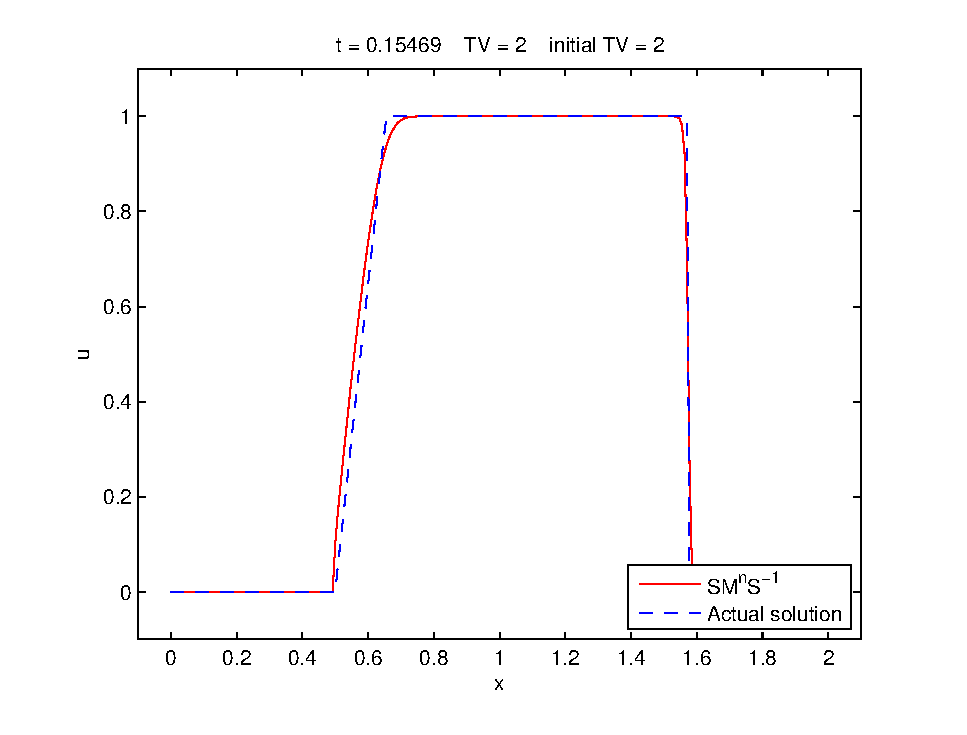
\includegraphics[scale=0.7]{Pictures/burgers_discont_tvd.eps}} \\
    \subfloat[$\sigma = 2.2$]{\label{fig5.4b}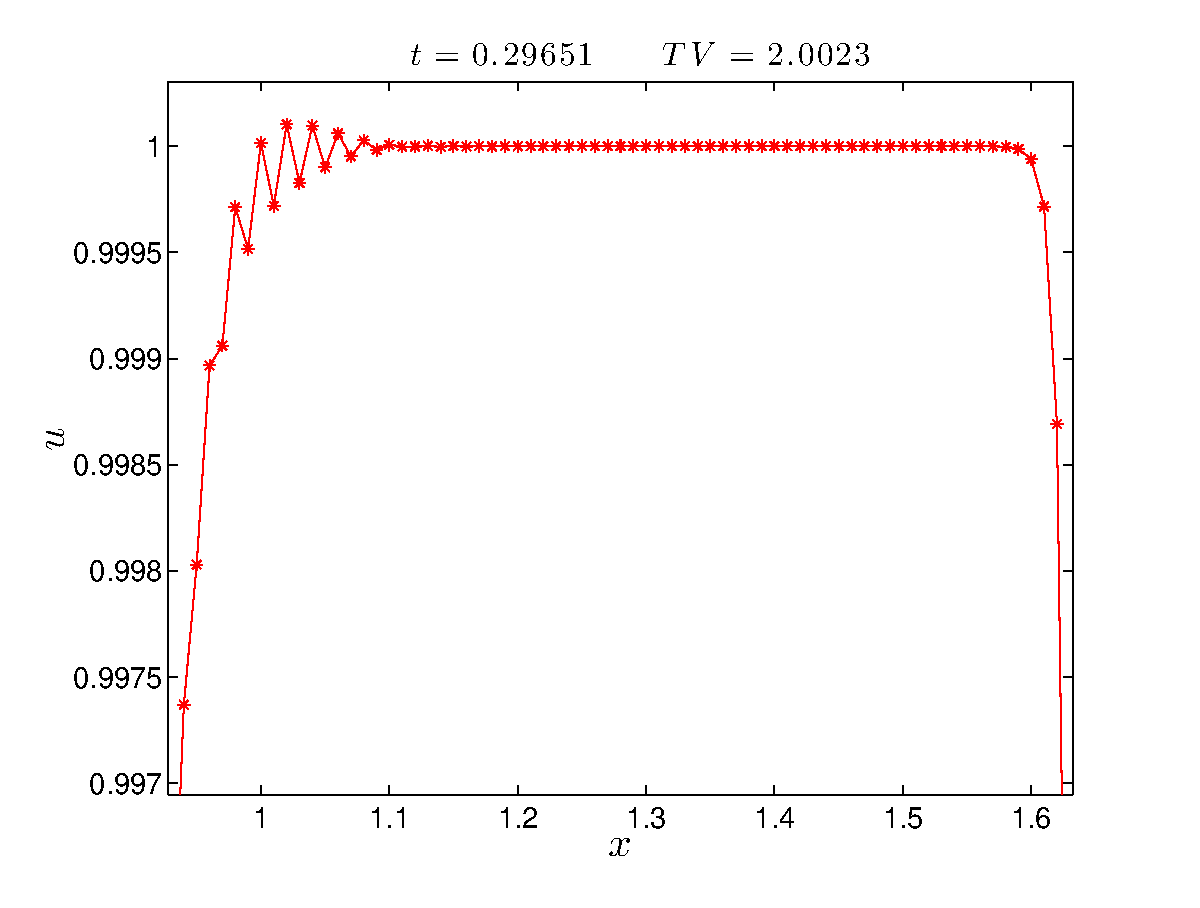
\includegraphics[scale=0.7]{Pictures/burgers_discont_no_tvd.eps}}
    \caption{Solution of Burger's equation with discontinuous initial data, using a $ SM^{n}S^{-1} $ scheme, where $ M $ is SSPRK($ 5 $,$ 4 $,$ 2 $) method. The SSP coefficient is $ c = 1.97 $.}
    \label{fig5.4}
\end{figure}

\subsubsection{Buckley-Leverett equation}\label{subsubsec:B-L}
